\section{AL\_\-TD  Class Reference}
\label{classAL__TD}\index{AL_TD@{AL\_\-TD}}
{\tt \#include $<$dil2al.hh$>$}

Inheritance diagram for AL\_\-TD::\begin{figure}[H]
\begin{center}
\leavevmode
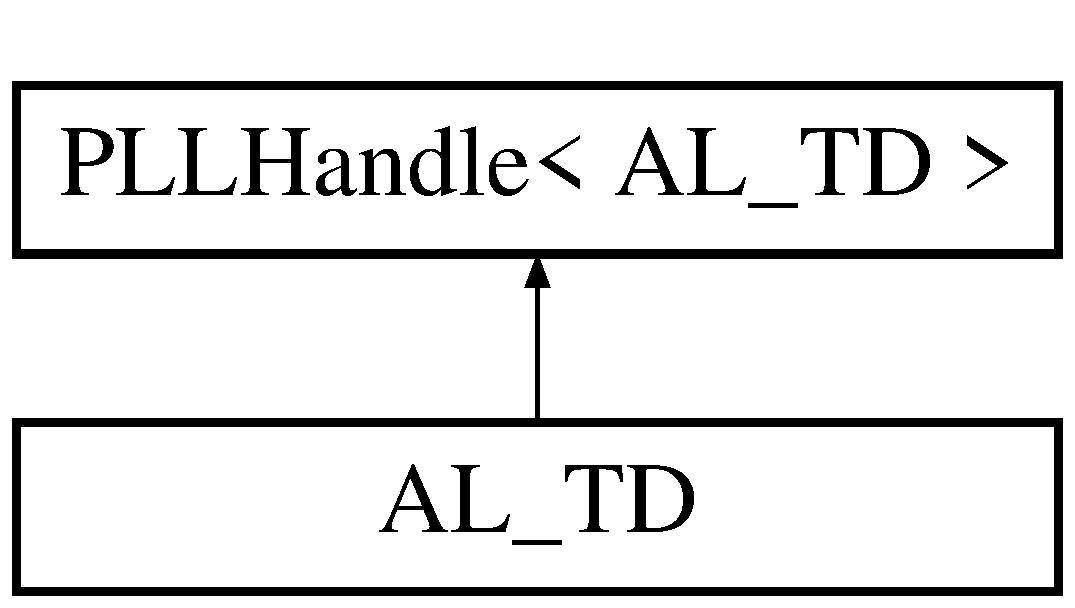
\includegraphics[height=2cm]{classAL__TD}
\end{center}
\end{figure}
\subsection*{Public Methods}
\begin{CompactItemize}
\item 
{\bf AL\_\-TD} ({\bf DIL\_\-entry} \&d)
\item 
{\bf $\sim$AL\_\-TD} ()
\item 
AL\_\-TD $\ast$ {\bf operator[$\,$]} (int n)
\item 
{\bf DIL\_\-entry} $\ast$ {\bf DE} () const
\item 
{\bf operator DIL\_\-entry $\ast$} () const
\end{CompactItemize}
\subsection*{Protected Attributes}
\begin{CompactItemize}
\item 
{\bf DIL\_\-entry} $\ast$ {\bf de}
\end{CompactItemize}


\subsection{Constructor \& Destructor Documentation}
\index{AL_TD@{AL\_\-TD}!AL_TD@{AL\_\-TD}}
\index{AL_TD@{AL\_\-TD}!AL_TD@{AL\_\-TD}}
\subsubsection{\setlength{\rightskip}{0pt plus 5cm}AL\_\-TD::AL\_\-TD ({\bf DIL\_\-entry} \& {\em d})\hspace{0.3cm}{\tt  [inline]}}\label{classAL__TD_a0}




Definition at line 836 of file dil2al.hh.



\footnotesize\begin{verbatim}836 : de(&d) {}
\end{verbatim}\normalsize 
\index{AL_TD@{AL\_\-TD}!~AL_TD@{$\sim$AL\_\-TD}}
\index{~AL_TD@{$\sim$AL\_\-TD}!AL_TD@{AL\_\-TD}}
\subsubsection{\setlength{\rightskip}{0pt plus 5cm}AL\_\-TD::$\sim$AL\_\-TD ()\hspace{0.3cm}{\tt  [inline]}}\label{classAL__TD_a1}




Definition at line 838 of file dil2al.hh.



\footnotesize\begin{verbatim}838 {} 
\end{verbatim}\normalsize 


\subsection{Member Function Documentation}
\index{AL_TD@{AL\_\-TD}!DE@{DE}}
\index{DE@{DE}!AL_TD@{AL\_\-TD}}
\subsubsection{\setlength{\rightskip}{0pt plus 5cm}{\bf DIL\_\-entry}$\ast$ AL\_\-TD::DE () const\hspace{0.3cm}{\tt  [inline]}}\label{classAL__TD_a3}




Definition at line 841 of file dil2al.hh.



\footnotesize\begin{verbatim}841 { return de; }
\end{verbatim}\normalsize 
\index{AL_TD@{AL\_\-TD}!operator DIL_entry *@{operator DIL\_\-entry $\ast$}}
\index{operator DIL_entry *@{operator DIL\_\-entry $\ast$}!AL_TD@{AL\_\-TD}}
\subsubsection{\setlength{\rightskip}{0pt plus 5cm}AL\_\-TD::operator {\bf DIL\_\-entry} $\ast$ () const\hspace{0.3cm}{\tt  [inline]}}\label{classAL__TD_a4}




Definition at line 842 of file dil2al.hh.



\footnotesize\begin{verbatim}842 { return de; }
\end{verbatim}\normalsize 
\index{AL_TD@{AL\_\-TD}!operator[]@{operator[]}}
\index{operator[]@{operator[]}!AL_TD@{AL\_\-TD}}
\subsubsection{\setlength{\rightskip}{0pt plus 5cm}AL\_\-TD$\ast$ AL\_\-TD::operator[$\,$] (int {\em n})\hspace{0.3cm}{\tt  [inline]}}\label{classAL__TD_a2}




Definition at line 840 of file dil2al.hh.

References PLLHandle$<$ AL\_\-TD $>$::el().



\footnotesize\begin{verbatim}840 { return el(n); }
\end{verbatim}\normalsize 


\subsection{Member Data Documentation}
\index{AL_TD@{AL\_\-TD}!de@{de}}
\index{de@{de}!AL_TD@{AL\_\-TD}}
\subsubsection{\setlength{\rightskip}{0pt plus 5cm}{\bf DIL\_\-entry}$\ast$ AL\_\-TD::de\hspace{0.3cm}{\tt  [protected]}}\label{classAL__TD_n0}




Definition at line 833 of file dil2al.hh.

The documentation for this class was generated from the following file:\begin{CompactItemize}
\item 
{\bf dil2al.hh}\end{CompactItemize}
